\subsection{Ground Penetrating Radar}

\subsubsection{Fundamentals of GPR}

Ground Penetrating Radar (GPR) is a non-invasive subsurface sensing technique that detects buried objects by emitting electromagnetic (EM) waves and analyzing their reflections. A typical GPR system is consisted of a wideband antenna and an active sensor. The antenna emits EM waves into the ground, and reflections are captured where there is a contrast in dielectric properties, like between soil and a buried landmine~\cite{paik2002image}.

The presence and depth of subsurface objects are inferred from discontinuities in the round-trip signal. The time delay $\Delta t$ between transmission and reception is used to estimate the distance $R$ to the reflecting object by \( R = \frac{v \cdot \Delta t}{2}\) where $v$ is the wave velocity in the medium depending on soil properties~\cite{paik2002image}.

To visualize GPR data, three types of scans are commonly used: \textbf{A-scan}, \textbf{B-scan}, and \textbf{C-scan}. A-scans represent 1D reflections at a single point, showing signal amplitude versus time delay. B-scans combine a series of A-scans along a line to form a 2D cross-sectional view of the subsurface, while C-scans stitche together multiple adjacent B-scans to generate a volumetric 3D map of the ground. 

Figure~\ref{fig:gpr_coords} illustrates the 3D coordinate system used in GPR scanning. A-scans are taken vertically into the ground at positions $(x’, y’)$. Moving the sensor along the $x$-axis forms a B-scan, and sweeping across $y$-axis yields a C-scan. A sample B-scan image is shown in Figure~\ref{fig:gpr_bscan}, where hyperbolic reflection patterns indicate buried objects~\cite{paik2002image}.

\begin{figure}[h!]
    \centering
    \begin{subfigure}[b]{0.48\linewidth}
        \centering
        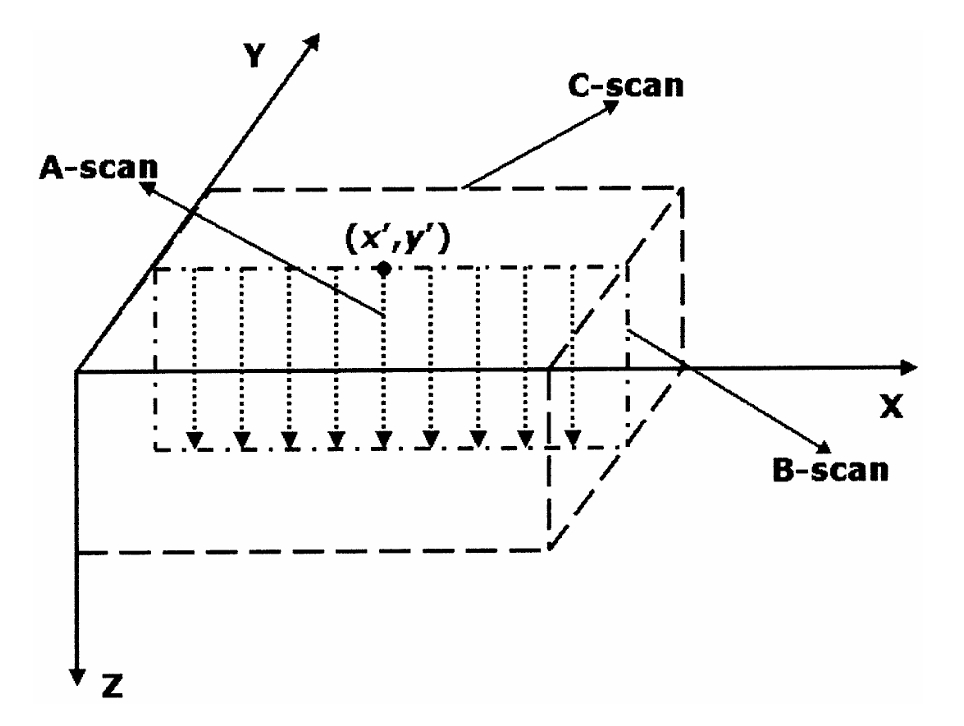
\includegraphics[height=5cm]{figs/Huirui/gpr_coords.png}
        \caption{Coordinate convention for GPR scanning.}
        \label{fig:gpr_coords}
    \end{subfigure}
    \hfill
    \begin{subfigure}[b]{0.48\linewidth}
        \centering
        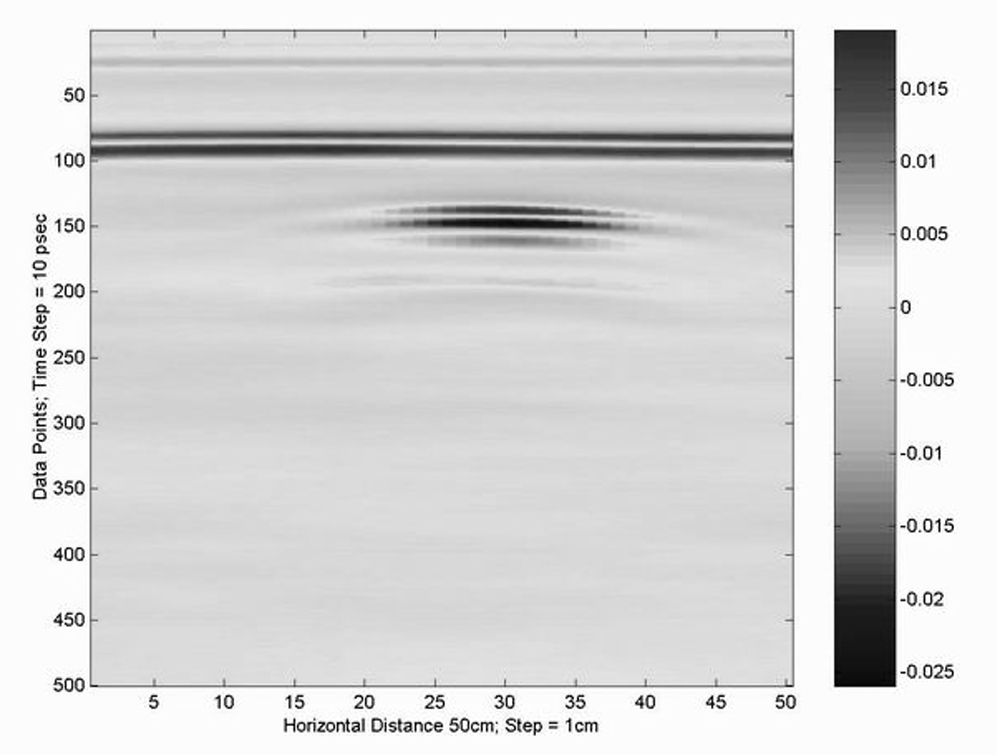
\includegraphics[height=5cm]{figs/Huirui/gpr_bscan.png}
        \caption{Example of a B-scan.}
        \label{fig:gpr_bscan}
    \end{subfigure}
    \caption{Visualization of GPR data acquisition and interpretation~\cite{paik2002image}.}
\end{figure}

Since our project focuses on localizing and estimating the depth of landmines rather than reconstructing their full 3D geometry, we collect and process only \textbf{B-scan} data from the UAV GPR platform.




\subsubsection{GPR Performance Factors}

The performance of a GPR system for UAV-based landmine detection depends on a variety of factors that influence its resolution, penetration depth, and system complexity. These include waveform generation methods, operating frequency and bandwidth, spatial resolution metrics, antenna design, signal processing techniques such as Synthetic Aperture Radar (SAR), and orientation of the radar with respect to the ground surface. This section outlines the main design parameters and discusses their implications for airborne GPR deployment.


\paragraph{Waveform Type}

The waveform type determines how GPR transmits and receives EM signals plays a critical role in determining resolution, hardware requirements, and system robustness. The three most common waveform types are summarized below:

\begin{itemize}
    \item \textbf{Impulse (pulsed)} GPR transmits ultra-short pulses with broad spectral content, enabling ultra-wideband (UWB) operation and high-resolution imaging. These systems are elatively simple and cost-effective but require high-speed analog-to-digital converters (ADCs) or subsampling receivers to process the wide bandwidth~\cite{chen2023ground,sipos2017drone}.

    \item \textbf{Frequency-Modulated Continuous Wave (FMCW)} GPR emits a continuous chirp signal with linearly increasing frequency over time. This approach offers better average transmitted power and improved SNR, but requires more complex hardware and is more vulnerable to phase noise and motion errors~\cite{burr2018design}.
    
    \item \textbf{Stepped-Frequency Continuous Wave (SFCW)}: GPR steps through discrete frequencies and collects reflections in the frequency domain. The data are then converted into time-domain signals via inverse Fourier transform. While achieving high SNR and reduced ADC requirements, SFCW systems often perform poorly in UAV applications due to weak ground coupling and strong surface reflections~\cite{tronca2018comparison}.
\end{itemize}


\paragraph{Centre Frequency, Bandwidth, Resolution, and Penetration Depth}

The center frequency and bandwidth of a radar signal are key parameters about the GPR system’s resolution and penetration depth. 

In general, lower frequencies (e.g., < 1 GHz) enhance penetration depth but limit resolution. Higher frequencies (e.g., > 2--3 GHz) improve resolution but attenuate quickly, especially in moist or conductive soils. For example, a GPR operating at 3~GHz may penetrate up to 0.5 m in dry soil, but only a few centimeters in wet environments~\cite{alqudsi2021review}. This trade-off is illustrated in Figure~\ref{fig:freq_tradeoff}, where increasing frequency improves resolution at the cost of reduced sensing depth.

The radar’s bandwidth, defined as the difference between the maximum and minimum frequencies $B = f_{\text{max}} - f_{\text{min}}$, determines the system’s range (or depth) resolution $\Delta r$, which is the ability to distinguish between objects at different depths along the same vertical axis. In free-space conditions where the wave velocity $v_p = c$ (the speed of light), the range resolution $\Delta r$ is approximated by: \(\Delta r = \frac{c}{2B}~\cite{alqudsi2021review}\)

Cross-range or lateral resolution $\Delta l$ defines the radar’s ability to distinguish adjacent objects at the same depth. It depends on the central wavelength $\lambda_c$, aperture size $L_{\text{ap}}$, and antenna-to-target distance $R$, and is approximated as: \(\Delta l = \frac{R \cdot \lambda_c}{L_{\text{ap}}}~\cite{alqudsi2021review}\)

\begin{figure}[h!]
    \centering
    \begin{subfigure}[t]{0.48\linewidth}
        \centering
        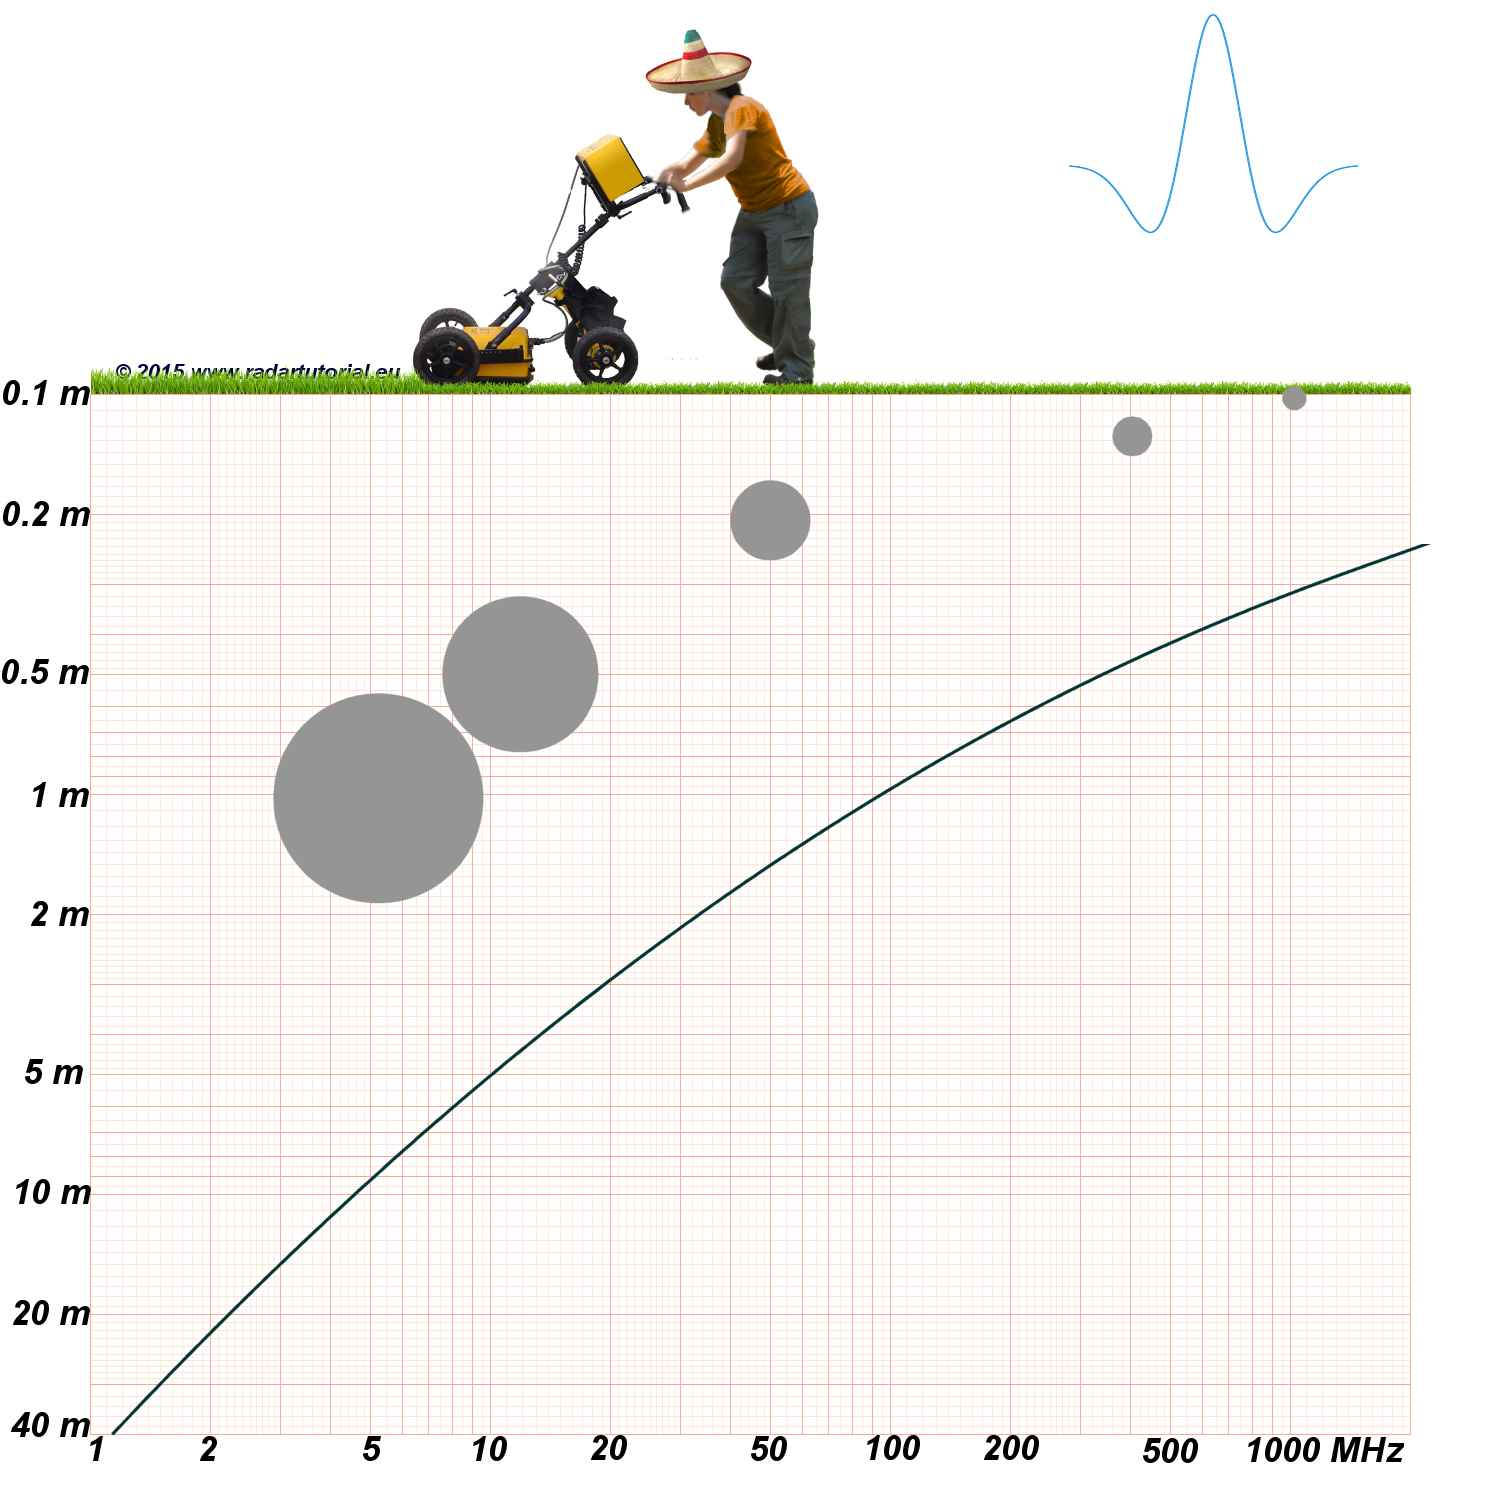
\includegraphics[height=4.2cm]{figs/Huirui/freq_tradeoff.png}
        \caption{Frequency–resolution vs. penetration depth trade-off\protect\footnotemark.}
        \label{fig:freq_tradeoff}
    \end{subfigure}
    \hfill
    \begin{subfigure}[t]{0.48\linewidth}
        \centering
        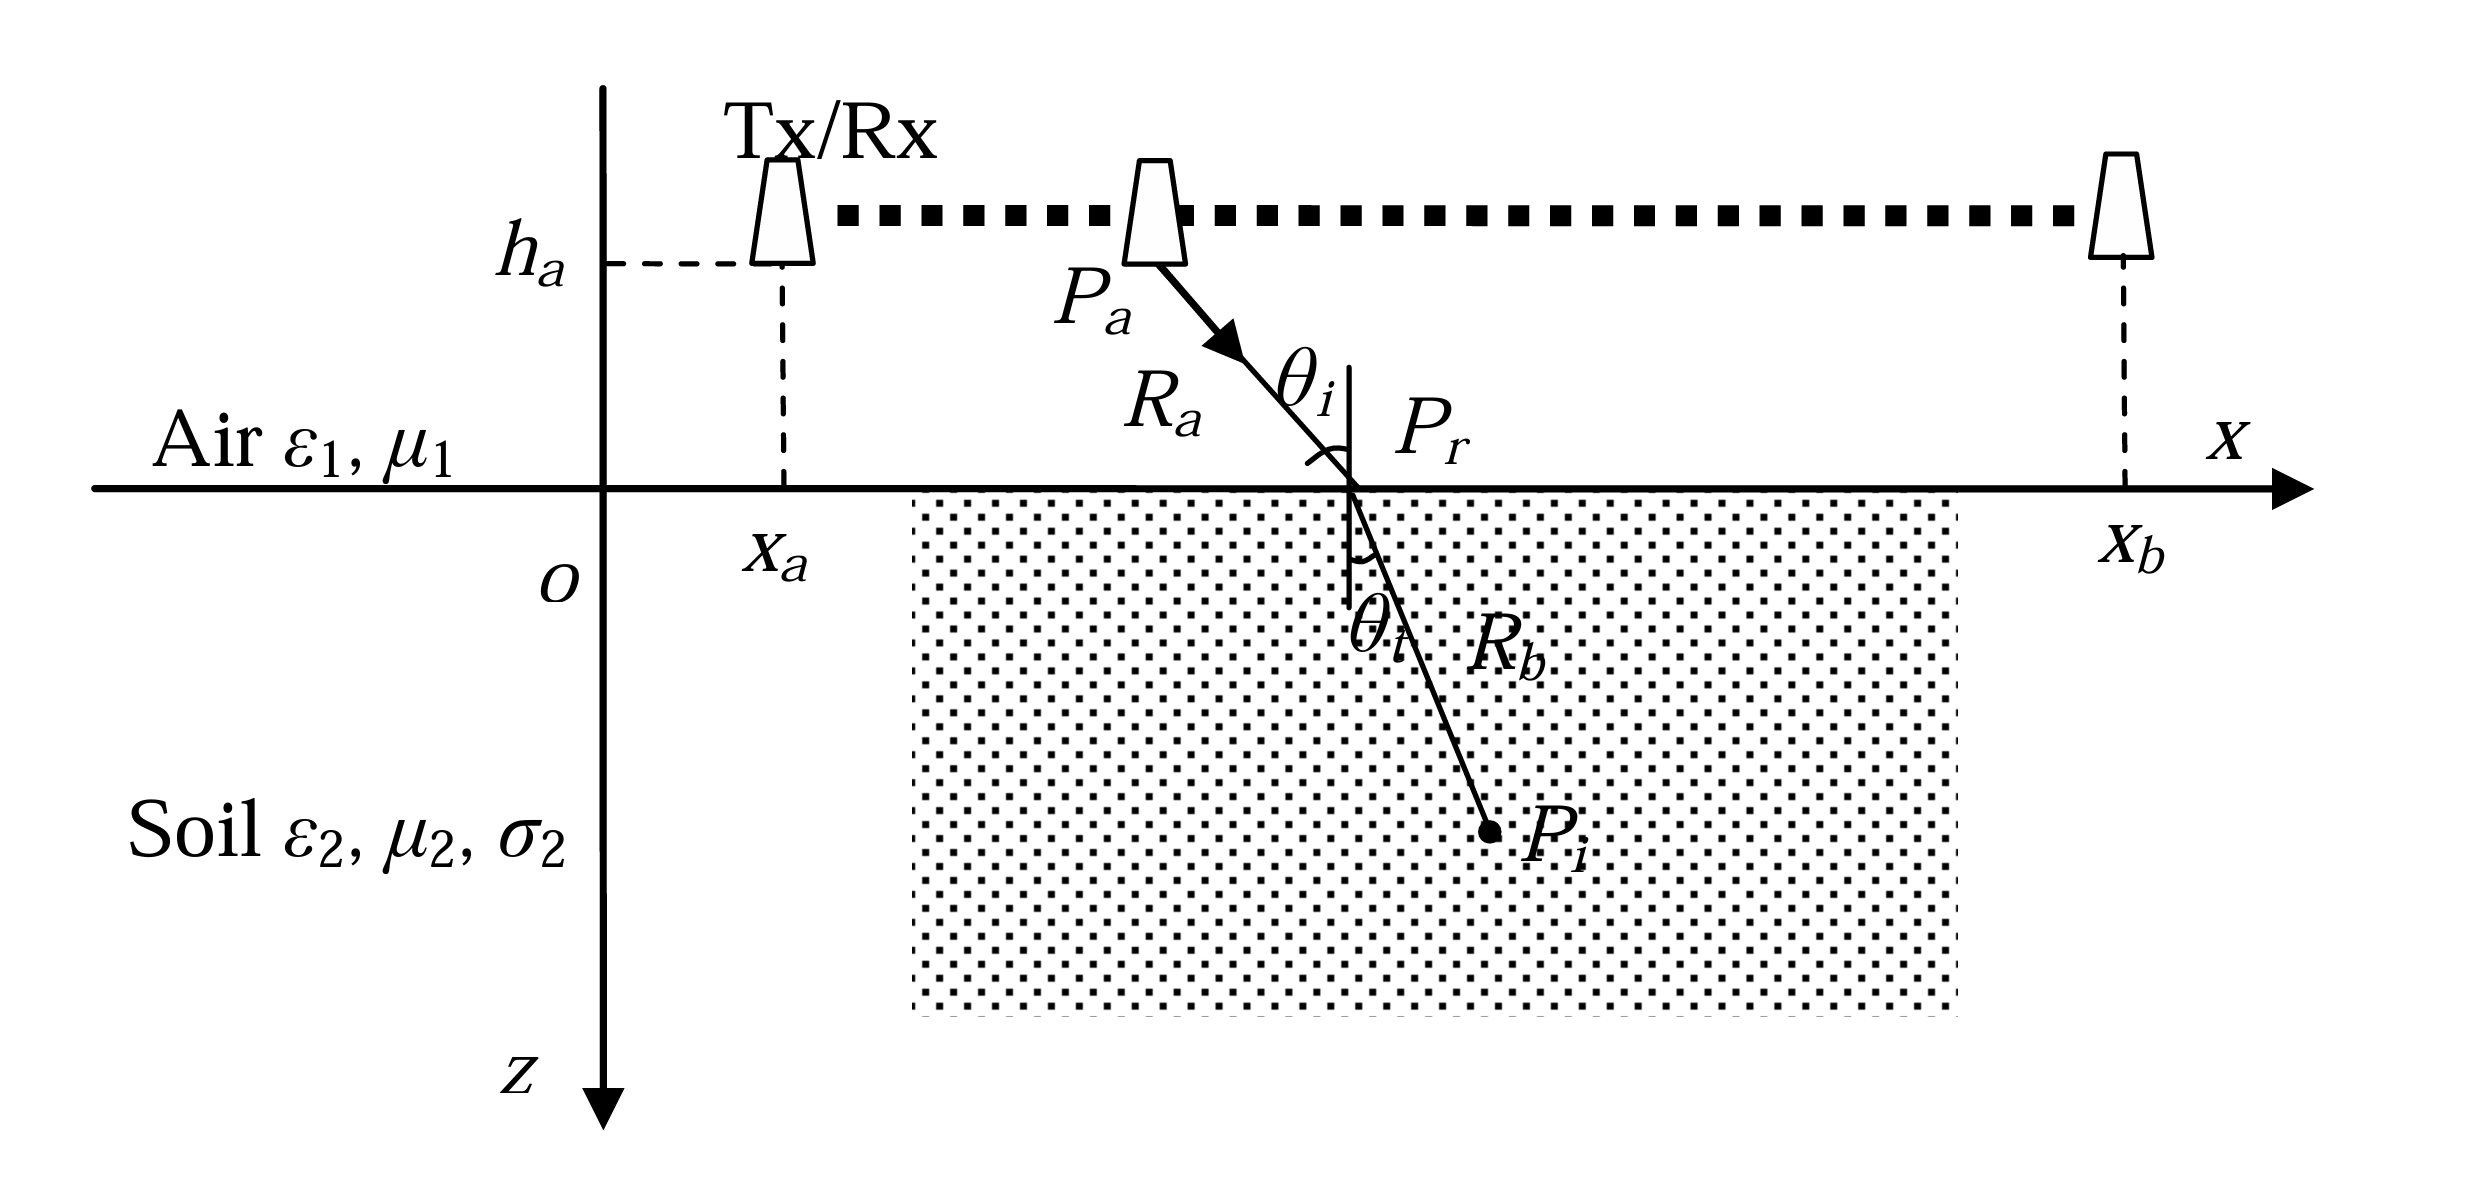
\includegraphics[height=4.2cm]{figs/Huirui/bp_geometry.png}
        \caption{Illustration of BP imaging geometry~\cite{lei2014multi}.}
        \label{fig:bp_geometry}
    \end{subfigure}
    \caption{Trade-offs and imaging geometry in UAV-based GPR.}
\end{figure}

\footnotetext{\url{www.radartutorial.eu}}


\paragraph{Synthetic Aperture Radar (SAR) Processing}

Traditional GPR systems have limited cross-range resolution due to the small sizes of antennas. SAR addresses this limitation by coherently integrating radar echoes collected along the UAV’s flight path, synthesizing a larger aperture, and significantly improving lateral resolution. This is especially beneficial for UAV-based GPR where antenna size and weight are constrained~\cite{alqudsi2021review}.

Among SAR algorithms, \textbf{Back-Projection (BP)} is particularly suited for UAV applications due to its robustness to irregular trajectories and non-uniform sampling. BP operates by summing radar echoes along computed time-delay curves for each focal point. As shown in Figure~\ref{fig:bp_geometry}, radar signals $e_1(x_p, t)$ are collected at multiple UAV positions $x_p$. The round-trip travel time $\tau_{m,n,p}$ from the transmitter to a target point $(x_n, z_m)$ and back is used to time-shift and coherently sum these signals by \(e_2(x_n, z_m) = \sum_{p=1}^{P} e_1(x_p, \tau_{m,n,p})\) and \(\tau_{m,n,p} = \frac{2R_a}{c} + \frac{2R_b}{v}\) where $R_a$ and $R_b$ are distances through air and soil respectively, $c$ is the speed of light, and $v$ is the wave velocity in soil. This delay-and-sum approach transforms hyperbolic reflections in conventional B-scans (like Figure~\ref{fig:gpr_bscan}) into focused point targets, improving subsurface interpretability. However, the method is computationally intensive and not ideal for real-time onboard processing~\cite{lei2014multi}.

SAR can operate in different beam-steering modes depending on coverage and resolution needs (Figure~\ref{fig:sar_modes}):

\begin{itemize}
    \item \textbf{Stripmap SAR} maintains a fixed beam relative to the UAV, illuminating a continuous swath as the platform moves forward, which offers a balance between area coverage and resolution~\cite{moreira2013tutorial}.
    \item \textbf{ScanSAR} periodically steers the beam to cover multiple adjacent swaths, increasing area coverage at the cost of reduced resolution~\cite{moreira2013tutorial}.
    \item \textbf{Spotlight SAR} keeps the beam focused on a single target area, maximizing resolution but limiting area coverage~\cite{moreira2013tutorial}.
\end{itemize}

\begin{figure}[h!]
    \centering
    \begin{subfigure}[b]{0.48\linewidth}
        \centering
        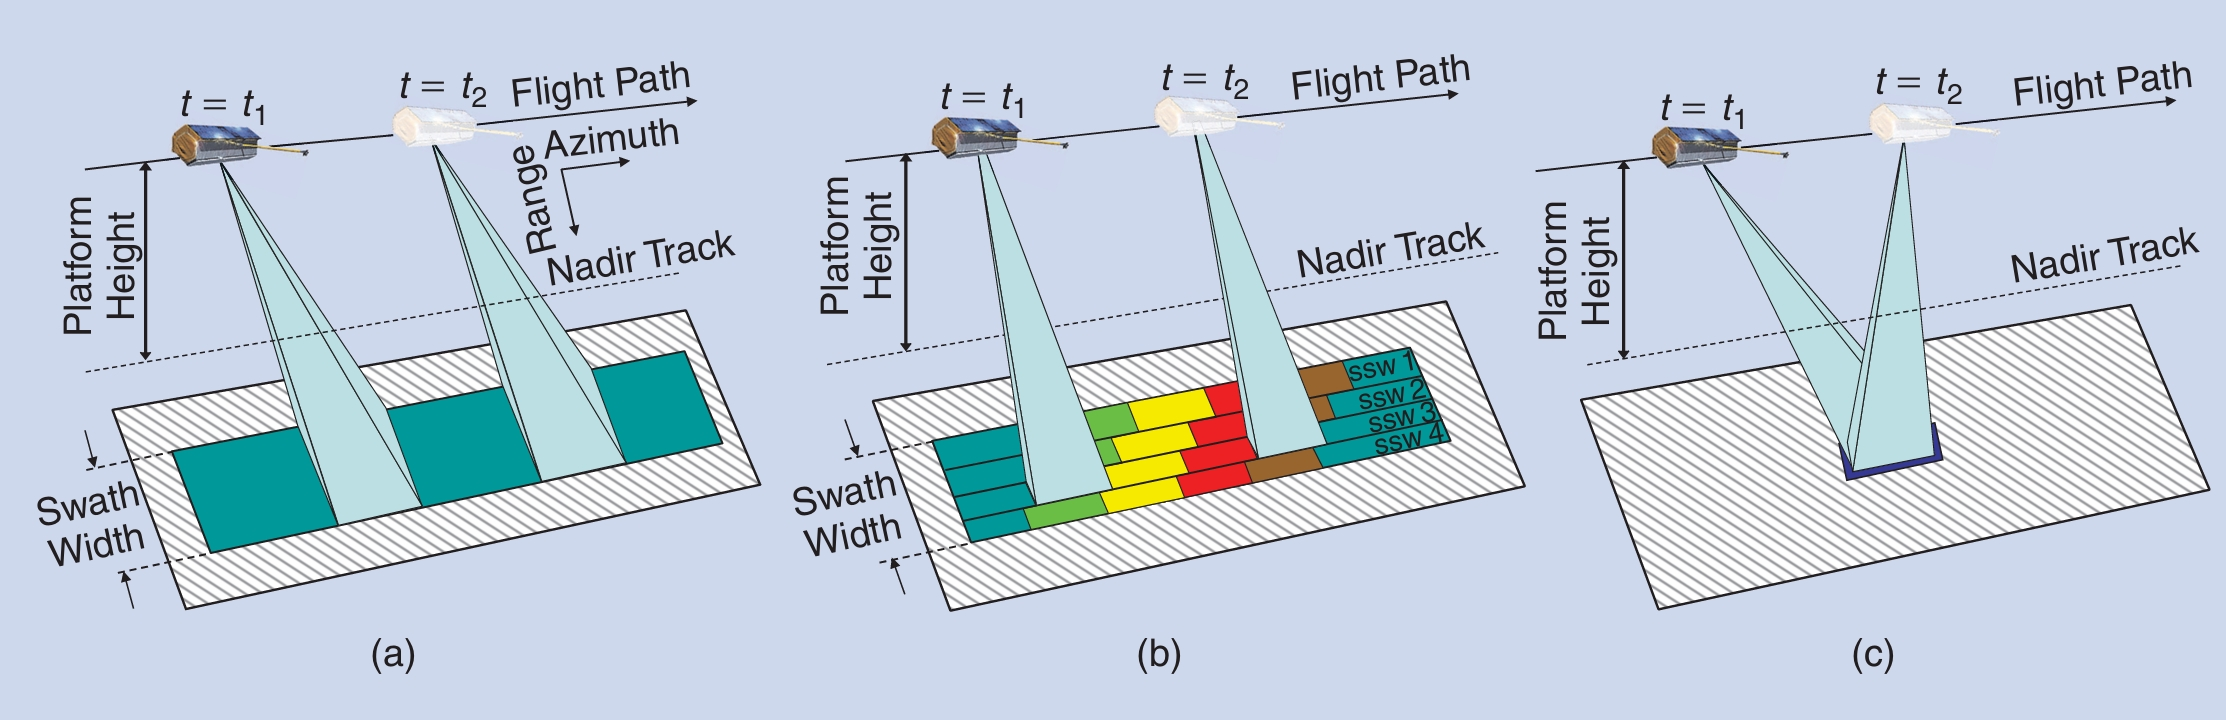
\includegraphics[height=3cm]{figs/Huirui/sar_modes.png}
        \caption{Different SAR operation modes~\cite{moreira2013tutorial}.}
        \label{fig:sar_modes}
    \end{subfigure}
    \hfill
    \begin{subfigure}[b]{0.48\linewidth}
        \centering
        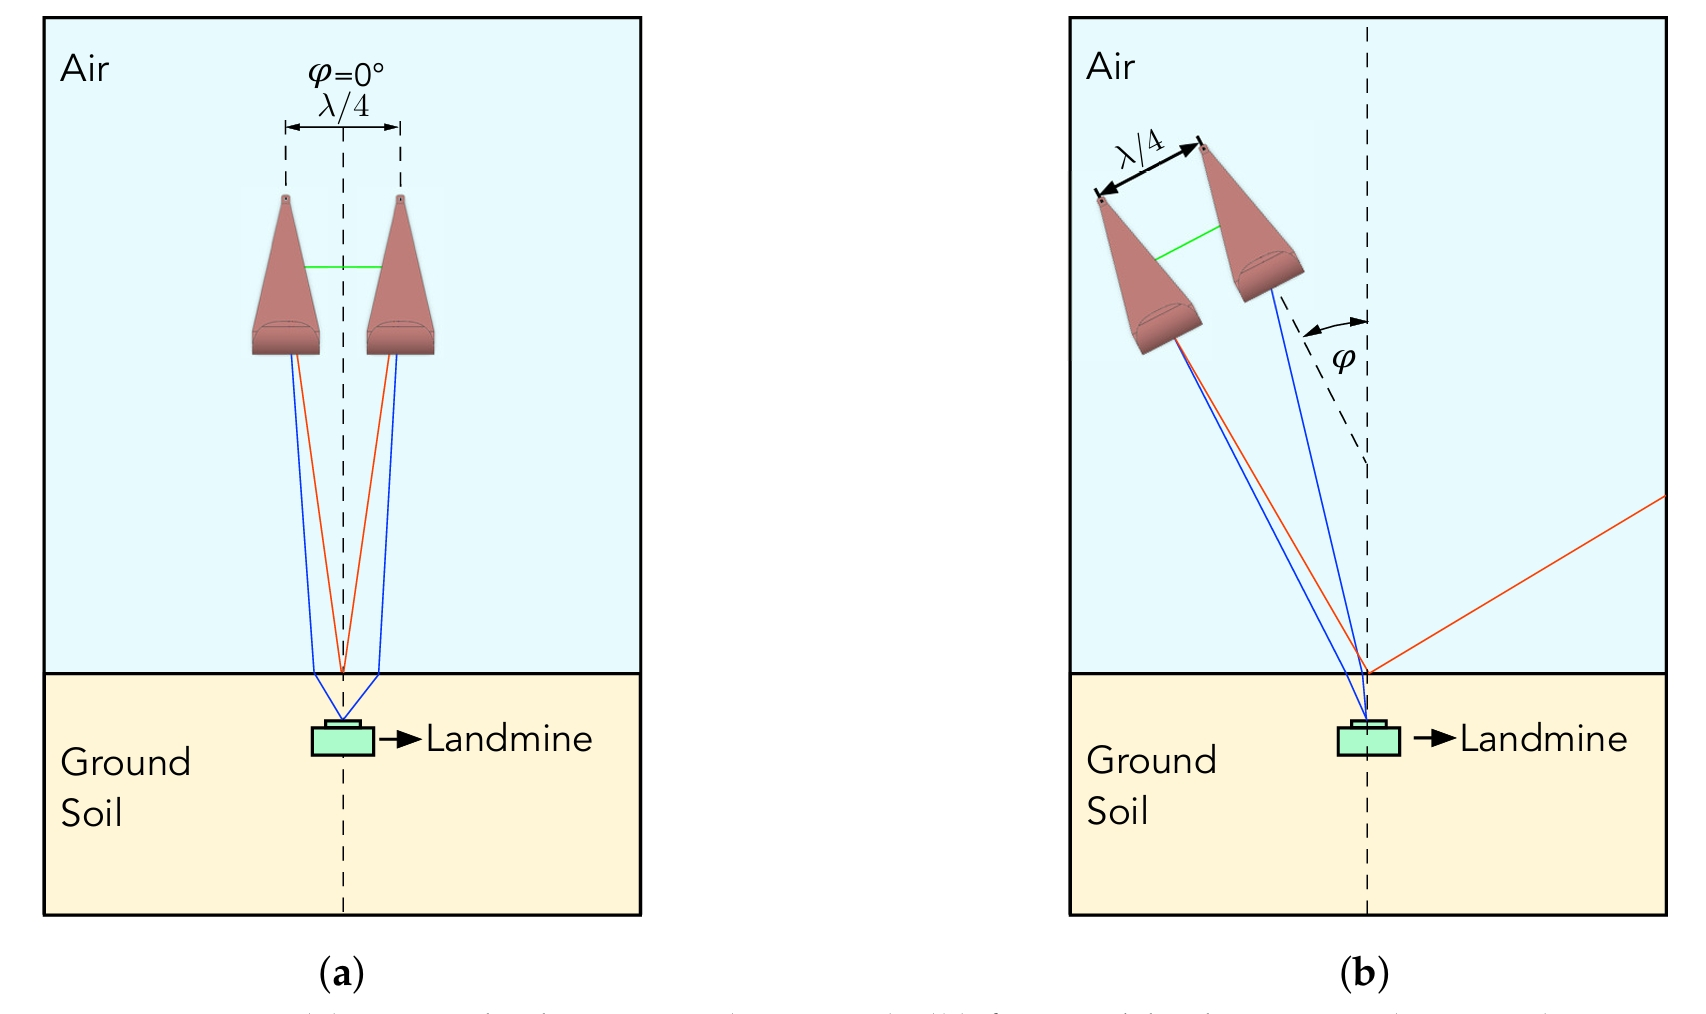
\includegraphics[height=3cm]{figs/Huirui/gpr_ori_modes.png}
        \caption{GPR orientations: DLGPR and FLGPR~\cite{vsipovs2020lightweight}.}
        \label{fig:GPR_Ori_modes}
    \end{subfigure}
    \caption{Illustration of SAR and GPR Orientation Modes}
    \label{fig:sar_gpr_modes}
\end{figure}

\paragraph{Radar Orientation}

The orientation of the GPR antenna on a UAV plays a critical role in determining both imaging performance and ease of integration. Two common configurations are illustrated in Figure~\ref{fig:GPR_Ori_modes}:

\begin{itemize}
    \item \textbf{Forward-Looking (FLGPR) or Side-Looking} emits waves obliquely into the ground, which reduces surface clutter. However, it receives weak backscattered signals from buried objects, requiring high dynamic range receivers and precise beam alignment~\cite{garcia2020airborne}.

    \item \textbf{Down-Looking (DLGPR)} points antennas perpendicularly toward the ground, maximizing reflected signal strength from targets but becoming more sensitive to surface clutter~\cite{garcia2020airborne}.
\end{itemize}


\paragraph{Antenna Size}

The physical size of a GPR antenna is closely linked to the operating frequency, with lower frequencies requiring larger antennas. A rough estimate of the minimum antenna length is given by: \(L_{\text{antenna}} \approx \frac{\lambda_{\text{min}}}{2}\), where $\lambda_{\text{min}}$ is the wavelength of the minimum GPR frequency~\cite{burr2018design}.

This relationship introduces a trade-off between penetration depth and physical size: lower frequencies penetrate deeper but require larger antennas, which may exceed the payload and form-factor limits of UAV platforms~\cite{alqudsi2021review}.



\subsubsection{GPR System Design}

While numerous GPR architectures have been explored in previous research, most high-performance UAV-based landmine detection systems rely on custom radar platforms. These typically incorporate Software-Defined Radio (SDR), customized waveform generators, and advanced antenna arrays to maximize their environmental adaptability, resolution, and penetration~\cite{cerquera2017uav}.

In contrast, the focus of our project is to demonstrate the feasibility of integrating GPR within a layered, multi-UAV landmine detection framework. Given the constraints of time, budget, and hardware development, we propose the use of a COTS impulse GPR system for our initial implementation.

We select the \textbf{SPH Engineering Zond Aero 1000 MHz GPR} (~1.8~kg\footnote{\label{Zond}\url{https://cdn.shopify.com/s/files/1/0596/9451/4353/files/RadSys_Zond_Aero_1000_NG_datasheet.pdf?v=1732295405}}). It operates in the 600–1300~MHz band with a center frequency of 1~GHz\textsuperscript{\ref{Zond}}, offering reasonable balance between resolution and penetration. Unlike high-frequency systems that offer fine detail at shallow depths, this system prioritizes deeper penetration—essential for detecting mines in compact or moist soils. Although its vertical resolution (around 10--15~cm) may not allow precise depth estimation, this is acceptable for our use case, where the primary goal is to confirm the existence rather than reconstruct detailed object geometry of the buried landmines.

The system uses a \textbf{DLGPR} configuration, maximizing reflected signal power from targets and simplifies hardware integration. While DLGPR does introduce surface clutter due to strong air–ground reflections, it can be mitigated through signal processing techniques such as Singular Value Decomposition (SVD) and migration algorithms ~\cite{garcia2024comparison}. Furthermore, DLGPR is the most widely adopted orientation in past UAV-GPR applications, supporting its practical reliability ~\cite{alqudsi2021review}.

To improve lateral resolution and compensate for the limited range resolution of our low-frequency radar, we apply SAR processing in \textbf{Stripmap} mode using a \textbf{BP} algorithm. This enables continuous scanning without beam steering, reducing UAV control complexity. BP processing is unaffected by trajectory deviations and achieves improved image focusing. Real-time processing is avoided due to the computational cost of BP; instead, raw B-scans will be geo-referenced using centimeter-level GNSS and IMU data and processed offline after each flight.


This system architecture based on a down-looking COTS impulse radar at low-frequency operation with offline SAR processing provides a realistic and effective foundation for our system’s initial deployment. It balances feasibility with performance, while leaving room for future upgrades such as real-time SDR control or custom radar development in subsequent project phases.



\subsubsection{Flight Configuration}

In our system, the GPR drone is designed to fly at an altitude of approximately 2 meters. This low flight height ensures a balance between maximizing power coupling into the ground and maintaining safe clearance for autonomous operations. The selected altitude is consistent with previous DLGPR studies on UAV landmine detection ~\cite{schartel2018uav,alqudsi2021review}.

As illustrated in Figure~\ref{fig:swath_geometry}, for our DLGPR system ($\alpha = 90^\circ$), assuming a beamwidth of $\theta = 45^\circ$, the effective swath width $W$ can be derived geometrically as \(W = 2H \cdot \tan\left(\frac{\theta}{2}\right)\). For $H = 2$~m,  $W = 1.65$~m. This value defines the effective width of ground coverage per flight strip.

\begin{figure}[H]
    \centering
    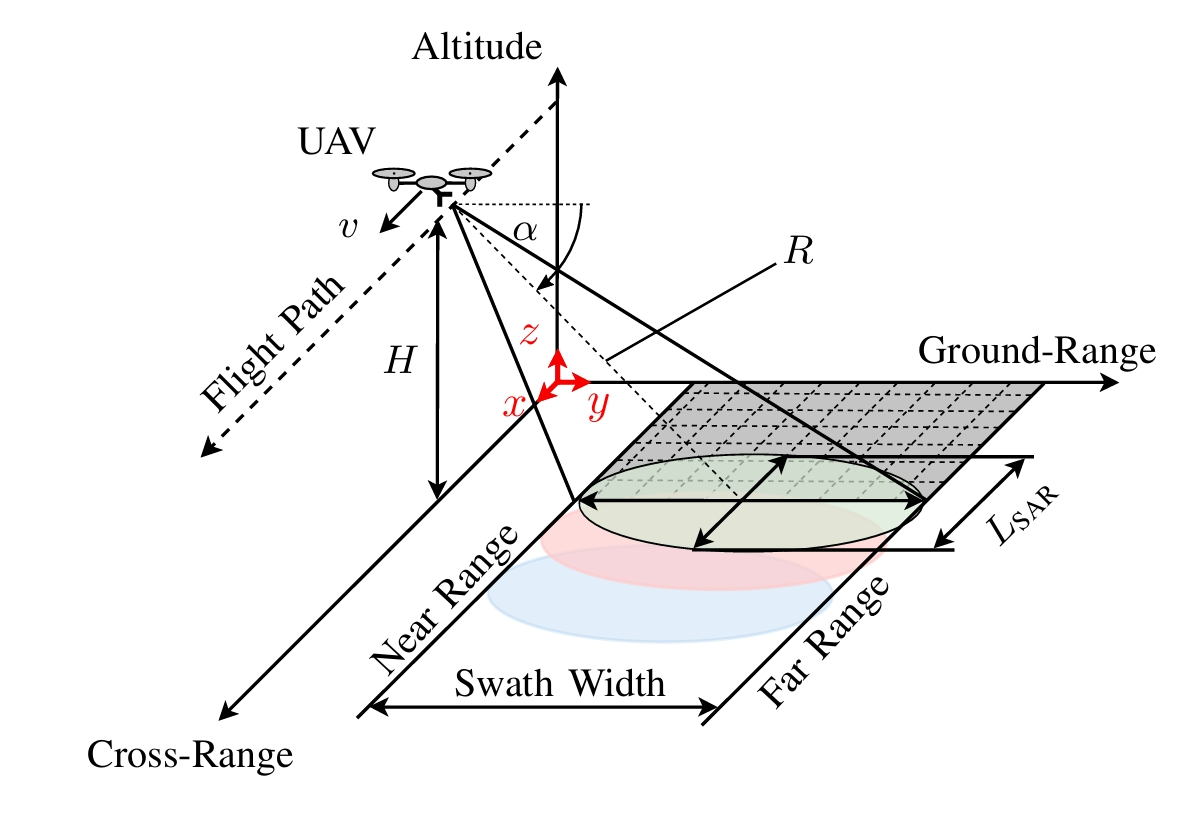
\includegraphics[height=5cm]{figs/Huirui/gpr_swath}
    \caption{Illustration of the stripmap SAR geometry.~\cite{schartel2018uav}.}
    \label{fig:swath_geometry}
\end{figure}

To enable effective SAR reconstruction using the BP algorithm, radar acquisition points must satisfy the Nyquist sampling rate, which requires that the maximum spacing $\Delta x$ between successive measurements does not exceed half the wavelength corresponding to the system's maximum radar frequency: \(\Delta x \leq \frac{\lambda_{\text{min}}}{2}\)~\cite{9758040}.

For our system with a maximum operating frequency of 1.3~GHz, the minimum wavelength is approximately 23~cm, resulting in a maximum sampling interval of \textbf{11.5~cm}. Given the estimated thermal camera coverage of 9 m × 7 m mentioned in section before, assuming a zig-zag path with overlapping swath like Figure~\ref{fig:swath_geometry}, a total of \textbf{332 points} are required to fully sample one thermally flagged region. 